
%---------------------------------------------------------------
% The "*" following chapter or section commands omits chapter/
% section numbers.  It also does not include the chapter/section
% in the table of contents -- the \addcontentsline can be used
% to manually force its entry.
%---------------------------------------------------------------

%\chapter*{Introduction}
%\addcontentsline{toc}{chapter}{Introduction}
\chapter{Introduction} \label{ch0}

The continued reduction of the transistor feature size has led to the increase in the vulnerability of modern circuits to error. This effect, in turn, has made modern circuits more susceptible to radiation induced errors in space and terrestrial environments. A radiation induced error, commonly referred to as a soft error, occurs when a high energy particle from space or packaging strikes a transistor. Shown in Fig. \ref{strike}, the particle arrives externally and deposits energy in the active volume generating electron-hole pairs. This creates a new diffusion region that could allow a non-conducting device to temporarily conduct current. The mechanism causes a temporary voltage pulse, referred to as a single event transient (SET) to occur at the device. If the SET occurs in combinational logic it may propagate to a memory element causing an error in the system. Furthermore, the error can occur in the memory element causing the stored data to be corrupted.

\begin{figure}[!htbp]
	\centering
	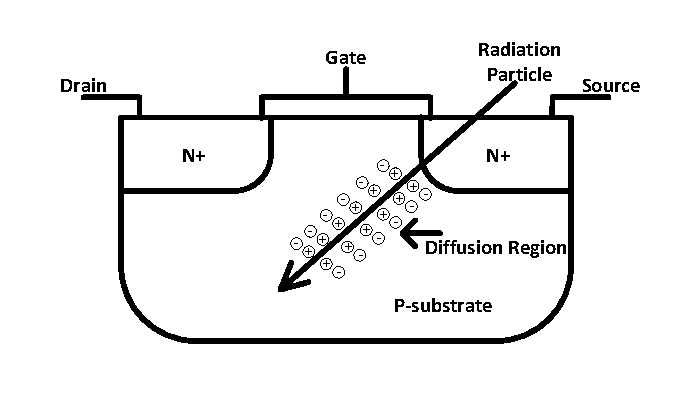
\includegraphics[width=0.50\linewidth]{Figures/StrikeFig}
	%where an .eps filename suffix will be assumed under latex, 
	%and a .pdf suffix will be assumed for pdflatex; or what has been declared
	%via \DeclareGraphicsExtensions.
	\caption{A energetic particle creating electron-hole pairs in a transistor.}
	\label{strike}
\end{figure} 

In Chapter \ref{ch1} the radiation effect on memory elements will be discussed. If a memory element loses its value due to a strike by a single particle, this is referred to as a single event upset (SEU). Additionally, due to the constant scaling down of the feature size, a single particle can also strike two transistors simultaneously which is referred to as a double node upset (DNU). Fig. \ref{DNUStrike} gives a diagram of a SEU tolerant latch to demonstrate the DNU phenomenon. In the diagram, radiation is denoted as a high energy particle which passes through two transistors on a DICE latch \cite{DICE}. In the case of a SEU, the DICE latch would normally be able to tolerate the error. As can be observed, the particle passes through two transistors causing the respective nodes to switch from ``1" on the first node to ``0" and from ``0" to ``1" on the second node. The upset of both nodes drives the remaining two nodes to an erroneous value. This observance is alarming since it signals that current designs are not sufficient for future processes. In turn, this provides a need for new memory element designs that can tolerate DNUs. 

\begin{figure}[!htbp]
	\centering
	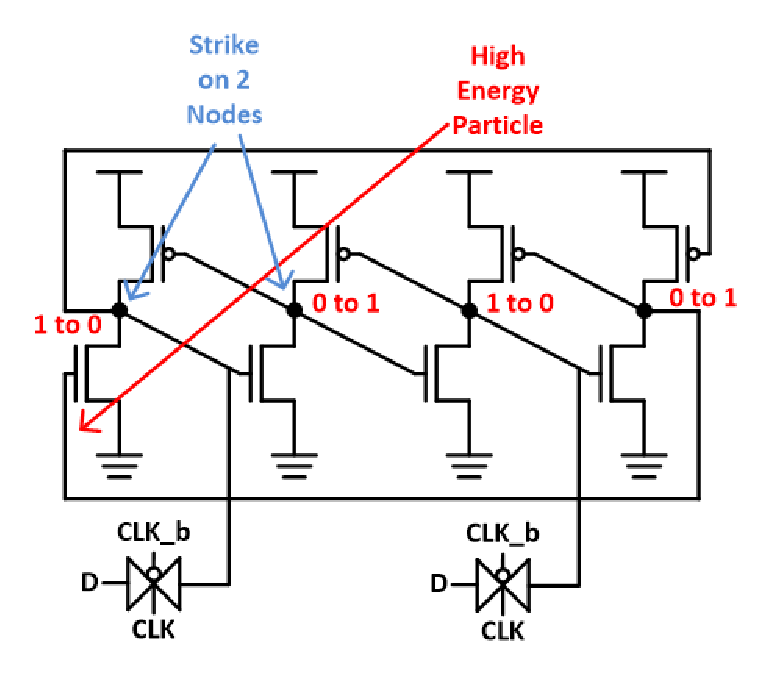
\includegraphics[width=0.45\linewidth]{Figures/StrikeonDICE}
	%where an .eps filename suffix will be assumed under latex, 
	%and a .pdf suffix will be assumed for pdflatex; or what has been declared
	%via \DeclareGraphicsExtensions.
	\caption{A particle striking two node concurrently causing a double node upset.}
	\label{DNUStrike}
\end{figure} 

In addition, many modern circuit designs employ a technique referred to as clock gating. Clock gating is defined as setting the clock to a constant value thus reducing the power consumed. Use of clock gating may lead to cases where the current state held by the memory element must be held for many clock cycles. This phenomenon leads to a much longer than normal vulnerable window in which an improperly hardened device may lose the stored value. While there are existing DNU tolerant designs \cite{Inter,DNCS,HSMUF}, these designs move to a high impedance state after a DNU. If a DNU occurs while the latch is gated, the voltages within the latch may degrade thus losing the stored value. In Chapter \ref{ch1}, the aim is to alleviate this problem by providing an efficient design that is capable of recovering all nodes after a DNU occurs. This, in effect, guarantees that the data will be held even if the latch is struck by a DNU while gated.

In addition to the effects on memory elements, accurate approximation of the error rate of a combinational circuit is also important. The goal of combinational circuit simulation is the accurate estimation of the soft error rate (SER). In Chapters \ref{ch2} and \ref{ch3} of this work, the focus is on the evaluation of the SER using near exact estimation methods on combinational circuits. Typically, this type of simulation entails the estimation of the resulting pulse shape when a particle strikes a transistor and during pulse propagation, the determination of the Boolean functions that allow the pulse to propagate and the estimation of the latching characteristics at an output flip-flop. Through accurate computation of the aforementioned effects, the probability of the pulse reaching an output flip-flop is determined. Assume that the probability of an error reaching and being latched in a flip-flop at output \textit{i} of a circuit is represented as \textit{$P(O_i)$}, the particle hit rate in a particular area is given as \textit{$R_{PH}$}, the fraction of particle hits resulting in charge generation as \textit{$R_{eff}$} and \textit{$A_{cir}$} gives the area of the circuit. The equation for the SER at output \textit{$O_i$} is given below \cite{METSys}.

\begin{equation}\label{SER_eq}
SER_{O_i} = P(O_i) * R_{eff} * R_{PH} * A_{cir}
\end{equation}

The focus of all SER estimation simulators is the calculation of the term \textit{$P(O_i)$}. This is a difficult problem due to the presence of the following three masking factors: electrical masking, logical masking and temporal masking. Electrical masking deals with the calculation of the pulse shape as it propagates through the circuit. Logical masking is the estimation of the logical 1's and 0's and how they may mask the pulse. For example, if a NAND gate has a value of ``0" on an input, the pulse will not propagate since the output will be held to a ``1". Lastly, temporal masking involves the latching characteristics, specifically the set-up and hold times and how they relate to the pulse width and clock period, of the output flip flop. Accurate consideration of all three masking effects is crucial to accurate SER estimation.

Accurate consideration of the electrical masking effect is an important but often simplified component of SER estimation. The most common method to calculate the pulse shape, proposed in \cite{Omana_Trap} uses a linear ramp to approximate the rising and falling transitions and a straight line for the peak giving a trapezoidal shape. While this method executes quickly and is easy to implement, it does not accurately represent the realistic shape of the pulse. As can be observed in Fig. \ref{T_pulse}, a transient pulse does not take a trapezoidal shape in a real case. For this reason, accurate consideration of the pulse shape must consider the non-linear aspects of the pulse. In \cite{Accurate_Masking}, the authors proposed an enhanced pulse approximation method which is accurate within 5\% of HSPICE. However, their method has the drawback that it can only consider a single pulse arriving at a gate. This is problematic in modern circuit simulation due to the continued scaling of the feature size has increased the likelihood of a radiation particle generating two or more pulses simultaneously, referred to as a multiple event transient (MET).
In the case of a MET, the number of pulses within the circuit substantially increase leading to a higher likelihood of multiple pulses arriving a gate simultaneously as shown in Fig. \ref{G_pulse}. This trend implies that future soft error simulators must be able to accurately consider multiple pulses. In Chapter \ref{ch2} an enhanced analytical pulse approximation algorithm which can consider any number of concurrent input pulses is proposed.

\begin{figure}[!htbp]
	\centering
	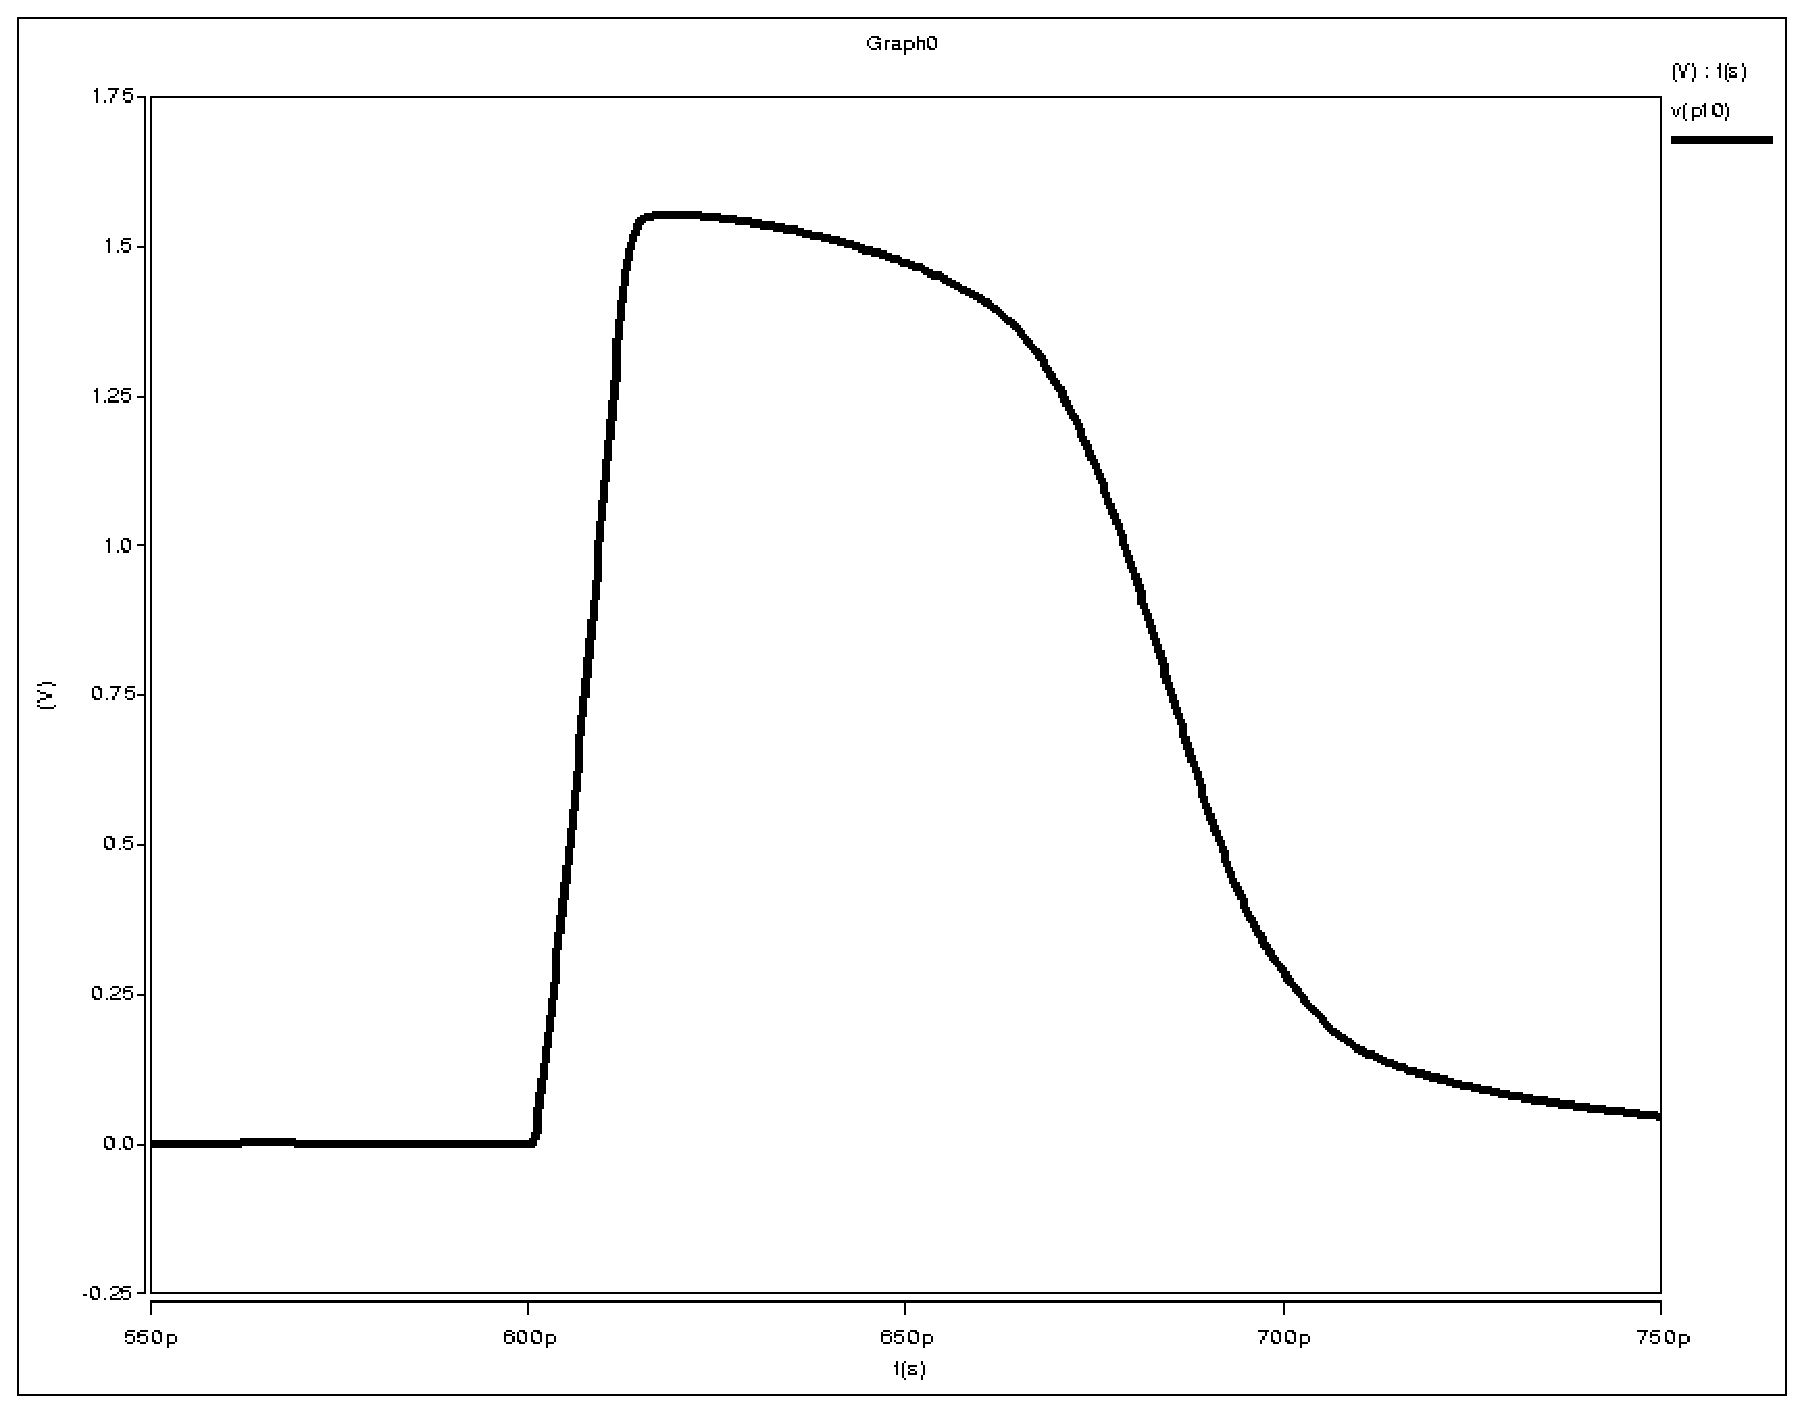
\includegraphics[width=0.45\linewidth]{Figures/Pulse_Shape}
	%where an .eps filename suffix will be assumed under latex, 
	%and a .pdf suffix will be assumed for pdflatex; or what has been declared
	%via \DeclareGraphicsExtensions.
	\caption{An example of a radiation induced transient pulse.}
	\label{T_pulse}
\end{figure} 

\begin{figure}[!htbp]
	\centering
	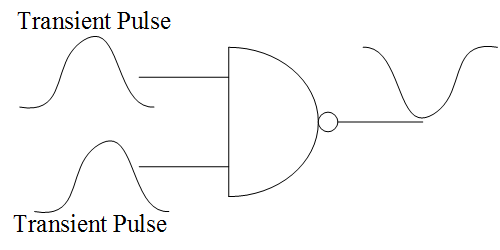
\includegraphics[width=0.45\linewidth]{Figures/gatepulse}
	%where an .eps filename suffix will be assumed under latex, 
	%and a .pdf suffix will be assumed for pdflatex; or what has been declared
	%via \DeclareGraphicsExtensions.
	\caption{Two pulses arriving at a gate input.}
	\label{G_pulse}
\end{figure} 

In addition to the electrical masking effect, the logical masking effect must also be accurately considered. Many existing methods use Monte Carlo based simulation which consists of either exhaustively apply all patterns or randomly applying a subset of patterns \cite{Accurate_Masking,PARAM_DESC,SEMM,SERA,SETA_LA}. While these methods are able to simulate with a very low memory overhead, they have an intractable execution time for circuits with more than 30 inputs. This problem is further compounded by the fact that due to the nearly infinite number of possible pulse durations and strike locations. To alleviate this issue, the authors in \cite{PTM} propose the use of probabilistic transfer matricies [PTM]. While the matricies do provide exact calculation of the logical masking effect, their memory usage blows up even for relatively small circuits. As an improvement to the use of PTMs, the use of decision diagrams have become more common \cite{FASER,MARS_C}. Decision diagrams offer an improved approach since they balance the cost of execution time and memory consumption. However, decision diagrams are not a perfect solution since, like PTMs, blow up if the circuit is sufficiently large. To solve this issue, the authors in \cite{FASER} proposed the use of partitioning to limit the size of the decision diagrams. The drawback with this approach is that each time the circuit is partitioned, additional error is added to the result. To ensure that the effect on the result is low, the number of partitions should be minimized based on the system resources available and the number of injected transient pulses.

In addition to the decision diagram blow-up problem, the simulator in \cite{MARS_C} uses algebraic decision diagrams (ADDs) which can have any numerical value as a terminating node. Their method also uses a simple pulse shape approximation algorithm in which pulses are approximated by on their width and magnitude. As stated previously, this type of approximation is not accurate since it does not consider the whole pulse shape. Due to the use of a simple approximation model, the ADDs are constructed such that the terminating node represents a pulse width or magnitude. The structures are then propagated by applying Boolean functions. A drawback with this approach is that if a more accurate pulse shape approximation model is used, the method in \cite{MARS_C} cannot properly store the pulse shape since more parameters are used for the pulse shape. Similar to \cite{MARS_C}, the tool in \cite{FASER} also does not use an accurate pulse approximation model. Furthermore, their tool does not have the means to consider convergent pulses or METs. In Chapter \ref{ch3}, these problems are addressed with a simulator that can determine the SER in the presence of METs using an accurate electrical masking model. 

In this dissertation, novel approaches to the aforementioned problems are proposed. In Chapter \ref{ch1}, a latch design is proposed which is capable of recovering all nodes after a DNU. This design has specific applications in circuits that employ clock gating. Chapter \ref{ch2} provides an enhanced analytical pulse approximation algorithm which can determine the output pulse shape when two pulses arrive at a gate input. The method is implemented and compared to existing algorithms and HSPICE. Chapter \ref{ch3} discusses a soft error simulator which employs partitioning and the pulse approximation mode in Chapter \ref{ch2}. Results are provided that compare the effect of partitioning to Monte Carlo simulation for the calculation of the SER.